%%%%%%%%%%%%%%%%%%%%%%%%%%%%%%%%%%%%%%%%%%%%%%%%%%%%%%%%%%%%%%%%%%
%%%%%%%%%%%%%%%%%%%%%%%%%%%%%%%%%%%%%%%%%%%%%%%%%%%%%%%%%%%%%%%%%%

\subsection{Architecture de l'\acrshort{os}}
Notre système d'exploitation a été conçu pour être utilisé sur un ordinateur
disposant d'un proceseur Intel de la famille x86. L'architecture x86 regroupe
plusieurs modes de fonctionnement. Les plus notables sont le \textit{real mode}
(16 bits), le \textit{protected mode} (32 bits) et le \textit{long mode} (64 bits).
Le mode réel n'est aujourd'hui plus utilisé mais tous les processeurs de la
famille x86, même modernes, démarrent dans ce mode avant de changer de mode.
Le système d'exploitation développé utilise le mode protégé. Cette architecture
se nomme \acrshort{IA-32} (Intel Architecture 32 bits, parfois appelée i386)
\cite{ref42}. \\

Le mode protégé offre deux mécanismes de gestion mémoire.
Ces mécanismes sont la segmentation et la pagination. Ils sont tous deux gérés
par l'\acrshort{os}. La gestion de la mémoire est traitée dans le chapitre \ref{memory}.
Un processeur Intel 32 bits peut aussi communiquer avec de nombreux périphériques.
Ceci se fait grâce à divers mécanismes comme les ports d'entrée/sortie ou
les interruptions matérielles. Un de ces périphériques est le disque dur de
l'ordinateur. Le disque dur doit avoir un système de fichiers pour être correctement
utilisable par l'\acrshort{os}. Par exemple, le système de fichiers utilisé
par Linux est ext2. Les périphériques et le système de fichiers sont décrits
dans les chapitres \ref{peripherals} et \ref{fs}. Enfin, le mode protégé fournit
un mécanisme de protection par niveau de privilèges. Ce mécanisme permet d'exécuter
du code destiné à l'utilisateur et de garantir la sûreté du système. Le chapitre
\ref{user} donne plus d'informations sur le mode utilisateur. Tous ces éléments
sont gérés par le noyau (\textit{kernel} en anglais) du système d'exploitation \cite{ref42}.

\begin{figure}[!h]
    \centering
    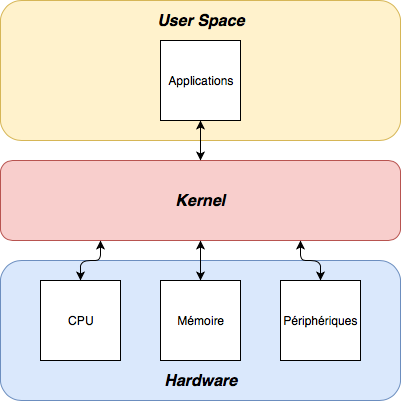
\includegraphics[scale=0.75]{images/kernel.png}
    \caption{Architecture du système d'exploitation}
    \label{os_arch}
\end{figure}

%%%%%%%%%%%%%%%%%%%%%%%%%%%%%%%%%%%%%%%%%%%%%%%%%%%%%%%%%%%%%%%%%%
%%%%%%%%%%%%%%%%%%%%%%%%%%%%%%%%%%%%%%%%%%%%%%%%%%%%%%%%%%%%%%%%%%

\subsection{Environnement de développement}
\label{sec:arch:host}
La machine utilisée pour le développement du projet est un MacBook Pro avec un
processeur Intel à 3 GHz. Il a quand même fallut utiliser une machine virtuelle
(VMware) utilisant Linux (Ubuntu 16.04.4 LTS) pour la compilation. Ce choix a été
fait car il existe beaucoup plus de documentation sur l'implémentation de systèmes
d'exploitation sur Linux que sur Mac. Bien que Mac \acrshort{os} soit un système
UNIX, les exécutables générés sur cet environnement n'ont pas le même format que
ceux générés sur Linux qui sont au format \acrshort{elf}. Ceci rend le développement
d'\acrshort{os} légèrement différent sur Mac \acrshort{os}. Linux est donc utilisé
pour la compilation et l'exécution du système d'exploitation. \\

Le code doit être compilé pour être exécutable sous une architecture \acrshort{IA-32}.
La compilation du code Rust est expliquée dans le chapitre \ref{rust_compil}. Certaines
parties du code du \textit{kernel} ont été écrites en assembleur car sont trop
bas niveau pour Rust. Il faut donc compiler le code Rust avec le code assembleur.
Tout le mécanisme de génération d'un \textit{kernel} est détaillé
dans le chapitre \ref{execution}. Dans ce projet, une machine
virtuelle est utilisée pour démarrer sur notre système d'exploitation. Cette machine
virtuelle est QEMU. Elle peut émuler plusieurs architectures dont l'architecture
i386 qui nous intéresse ici. QEMU peut démarrer sur un système d'exploitation depuis
un fichier \acrshort{iso}. La figure \ref{global_arch} illustre ce comportement \cite{ref42}.

\begin{figure}[!h]
    \centering
    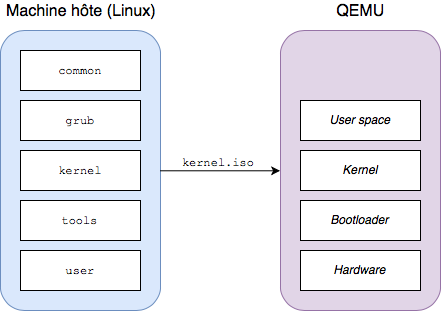
\includegraphics[scale=0.65]{images/global_arch.png}
    \caption{Architecture globale du projet}
    \label{global_arch}
\end{figure}

D'un côté nous avons la machine de développement (ou machine hôte) contenant tous
les fichiers servant à compiler le \textit{kernel}. De l'autre il y a QEMU qui
démarre le système d'exploitation à partir du \textit{kernel}. Les fichiers côté
machine de développement sont ordonnés d'une manière bien précise \cite{ref42}.

\begin{center}
	\scalebox{0.8}{
		\begin{tabular}{| l | l | }
			\hline
			Répertoire & Description \\ \hline
			\mintinline{text}{common} & Fichiers communs entre le \textit{kernel}
            et les applications utilisateurs \\ \hline
			\mintinline{text}{grub} & Fichiers de configuration du \textit{bootloader}
            \acrshort{grub} \\ \hline
			\mintinline{text}{kernel} & Code source du \textit{kernel} \\ \hline
			\mintinline{text}{tools} & Codes source des différents outils développés
            pour l'\acrshort{os} \\ \hline
			\mintinline{text}{user} & Codes source des des applications utilisateurs \\ \hline
		\end{tabular}
	}
    \captionof{table}{Structure du projet}
    \label{tab:project_struct}
\end{center}